\documentclass[FIPLY_base.tex]{subfiles}

%\author{Daniel Bersenkowitsch}
	
\begin{document}
	\subsection{Trainingsplan}
		Der Trainingsplan ist das Herzstück des Projekts. Wie in der Theorie beschrieben wird dieser mittels eines Algorithmus umgesetzt. 
	\subsubsection{Die Ansicht}
		 In der Trainingsplan Ansicht findet der Benutzer eine Liste mit allen existierenden Trainingsplänen vor. 
		 \begin{figure}[H]
		 	\begin{subfigure}[b]{0.3\textwidth}
				In der obigen Leiste befinden sich die Optionen \grqq{}hinzufügen\grqq{}, \grqq{}löschen\grqq{}, und die Knöpfe zum Exportieren eines ausgewählten Plans.
				
		 	\end{subfigure}
		 	\begin{subfigure}[b]{0.3\textwidth}
		 		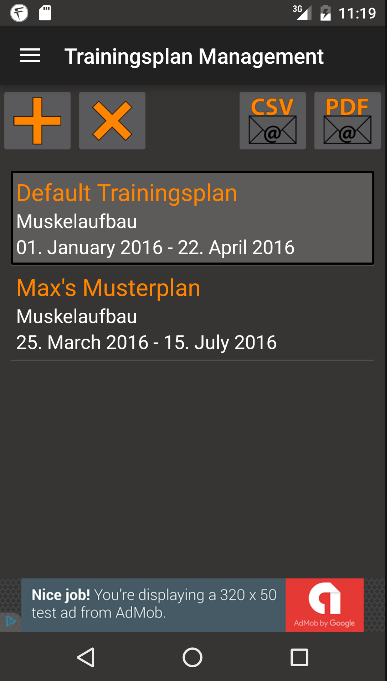
\includegraphics[scale=0.50]{img/tplanmgmt}
		 	\end{subfigure}
		 	\hfil
		 	\caption{Ansicht des Trainingspläne}
		 \end{figure}
\end{document}